\documentclass[10pt,twocolumn,letterpaper]{article}

%%%%%%%%% PAPER TYPE  - PLEASE UPDATE FOR FINAL VERSION
% \usepackage[review]{cvpr}      % To produce the REVIEW version
\usepackage{cvpr}              % To produce the CAMERA-READY version
%\usepackage[pagenumbers]{cvpr} % To force page numbers, e.g. for an arXiv version

% Include other packages here, before hyperref.
\usepackage{graphicx}
\usepackage{amsmath}
\usepackage{amssymb}
\usepackage{booktabs}
\usepackage[shortlabels]{enumitem}


% It is strongly recommended to use hyperref, especially for the review version.
% hyperref with option pagebackref eases the reviewers' job.
% Please disable hyperref *only* if you encounter grave issues, e.g. with the
% file validation for the camera-ready version.
%
% If you comment hyperref and then uncomment it, you should delete
% ReviewTempalte.aux before re-running LaTeX.
% (Or just hit 'q' on the first LaTeX run, let it finish, and you
%  should be clear).
\usepackage[pagebackref,breaklinks,colorlinks]{hyperref}


% Support for easy cross-referencing
\usepackage[capitalize]{cleveref}
\crefname{section}{Sec.}{Secs.}
\Crefname{section}{Section}{Sections}
\Crefname{table}{Table}{Tables}
\crefname{table}{Tab.}{Tabs.}


%%%%%%%%% PAPER ID  - PLEASE UPDATE
\def\cvprPaperID{*****} % *** Enter the CVPR Paper ID here
\def\confName{CVPR}
\def\confYear{2025}


\begin{document}

%%%%%%%%% TITLE - PLEASE UPDATE
\title{NTIRE 2025 Efficient SR Challenge Factsheet\\-title of the contribution-}

\author{
Shengyun Zhong\\
Northeastern University, USA\\
{\tt\small shengyunzhong2002@gmail.com}
\and
Mingyang Wu\\
Texas A\&M University, USA\\
{\tt\small mingyang@tamu.edu}
\and
Renjie Li\\
Texas A\&M University, USA\\
{\tt\small renjie@tamu.edu}
\and
Yushen Zuo\\
The Hong Kong Polytechnic University, Hong Kong\\
{\tt\small zuoyushen12@gmail.com}
\and
Zhengzhong Tu\\
Texas A\&M University, USA\\
{\tt\small tzz@tamu.edu}
}
\maketitle


\section{Introduction}

This factsheet template is meant to structure the description of the contributions made by each participating team in the NTIRE 2025 challenge on efficient image super-resolution. 

Ideally, all the aspects enumerated below should be addressed.
The provided information, the codes/executables and the achieved performance on the testing data are used to decide the awardees of the NTIRE 2025 challenge. 

Reproducibility is a must and needs to be checked for the final test results in order to qualify for the NTIRE awards. 

The main winners will be decided based on overall performance and a number of awards will go to novel, interesting solutions and to solutions that stand up as the best in a particular subcategory the judging committee will decided. Please check the competition webpage and forums for more details.

The winners, the awardees and the top ranking teams will be invited to co-author the NTIRE 2025 challenge report and to submit papers with their solutions to the NTIRE 2025 workshop. Detailed descriptions are much appreciated.

The factsheet, \href{https://github.com/Amazingren/NTIRE2025_ESR}{source codes/executables}, trained models should be sent to \textbf{all of the NTIRE 2025 challenge organizers (Yawei Li, Bin Ren, Nancy Mehta, and Radu Timofte)} by email.


\section{Email final submission guide}
\noindent \textbf{To:} \\
{yawei.li@vision.ee.ethz.ch} \\ 
{bin.ren@unitn.com} \\ 
{cshguo@gmail.com} \\
{zongwei.wu@uni-wuerzburg.de}\\
{timofte.radu@gmail.com}\\
\noindent \textbf{CC:} \\
your\_team\_members\\


Title: NTIRE 2025 Efficient SR Challenge - TEAM\_NAME - TEAM\_ID\\

To get your TEAM\_ID, please register at \href{https://docs.google.com/spreadsheets/d/11JuxcS78C6Gxc8B436L4Zk4_m5soHaTcw3cnF8h5ctE/edit?usp=sharing}{Google Sheet}. Please fill in your Team Name, Contact Person, and Contact Email in the first empty row from the top of the sheet.
% 
Body contents should include: 

\begin{enumerate}[a)]
    \item team name 
    
    \item team leader's name and email address 
    
    \item rest of the team members 
    
    \item user names on NTIRE 2025 CodaLab competitions 
    
    \item Code, pre-trained model, and factsheet download command, e.g. \texttt{git clone ...}, \texttt{wget ...}
    
    \item Result download command, e.g. \texttt{wget ...}
    
    \begin{itemize}
        \item Please provide different URLs in e) and f)
    \end{itemize}
\end{enumerate}



\noindent Factsheet must be a compiled pdf file together with a zip with .tex factsheet source files. Please provide a detailed explanation.


\section{Code Submission}

The code and trained models should be organized according to the \href{https://github.com/Amazingren/NTIRE2025_ESR}{GitHub repository}. This code repository provides the basis to compare the various methods in the challenge. \textbf{Code scripts based on other repositories will not be accepted.} Specifically, you should follow the steps below.
\begin{enumerate}
    \item Git clone \href{https://github.com/Amazingren/NTIRE2025_ESR}{the repository.}
    \item Put your model script under the \texttt{models} folder. Name your model script as \texttt{[Your\_Team\_ID]\_[Your\_Model\_Name].py}.
    \item Put your pretrained model under the \texttt{model\_zoo} folder. Name your model checkpoint as \texttt{[Your\_Team\_ID]\_[Your\_Model\_Name].[pth or pt or ckpt]}
    \item Modify \texttt{model\_path} in \texttt{test\_demo.py}. Modify the imported models.
    \item \texttt{python test\_demo.py}
\end{enumerate}
Please send us the command to download your code, e.g. \texttt{git clone [Your repository link]}
When submitting the code, please remove the LR and SR images in \texttt{data} folder to save the bandwidth.

\section{Factsheet Information}

The factsheet should contain the following information. Most importantly, you should describe your method in detail. The training strategy (optimization method, learning rate schedule, and other parameters such as batch size, and patch size) and training data (information about the additional training data) should also be explained in detail.

\subsection{Team details}

\begin{itemize}
\item Team name: TACO\_SR                                
\item Team leader: Shengyun Zhong                          
\item Address: 935N 72nd St, 98103, Seattle, WA, USA\\Phone: +1 (510)916-9891\\email: shengyunzhong2002@gmail.com
\item Rest of members: Mingyang Wu, Renjie Li, Yushen Zuo, Zhengzhong Tu      
\item Team URL: https://taco-group.github.io/                   
\item Affiliation:\\
      Shengyun Zhong: Northeastern University, USA \\
      Mingyang Wu: Texas A\&M University, USA \\
      Renjie Li: Texas A\&M University, USA \\
      Yushen Zuo: The Hong Kong Polytechnic University, Hong Kong \\
      Zhengzhong Tu: Texas A\&M University, USA
\item Affiliation of the team and/or team members with NTIRE 2025 sponsors: None
\item User names: ShelvinZhong \\
      Entries(development/validation phases): 6 \\
      Entries(testing phases): 2
\item Link to the codes/executables of the solution(s): https://github.com/ShelvinZhong/TenInOneSR\_EVAL
\end{itemize}

\subsection{Method details}

\textbf{Method. } The overall architecture of their network is showed in the Figure(a), inspired by SPAN~\cite{SPAN2024} and PFDNLite~\cite{NTIRE2024Report}. Motivated by the design of the Conv3XC module in SPAN, they introduce two additional parallel branches with varying channel expansion ratios, resulting in a novel convolution module termed TenInOneConv, which fuses multiple convolution kernels into a single equivalent kernel to improve inference efficiency. Furthermore, to enhance the model’s capability in capturing local texture and detail features, the LocalAttention module inspired by PFDNLite is integrated, allowing the network to better focus on informative regions within feature maps. 
\begin{figure}[t]
  \centering
  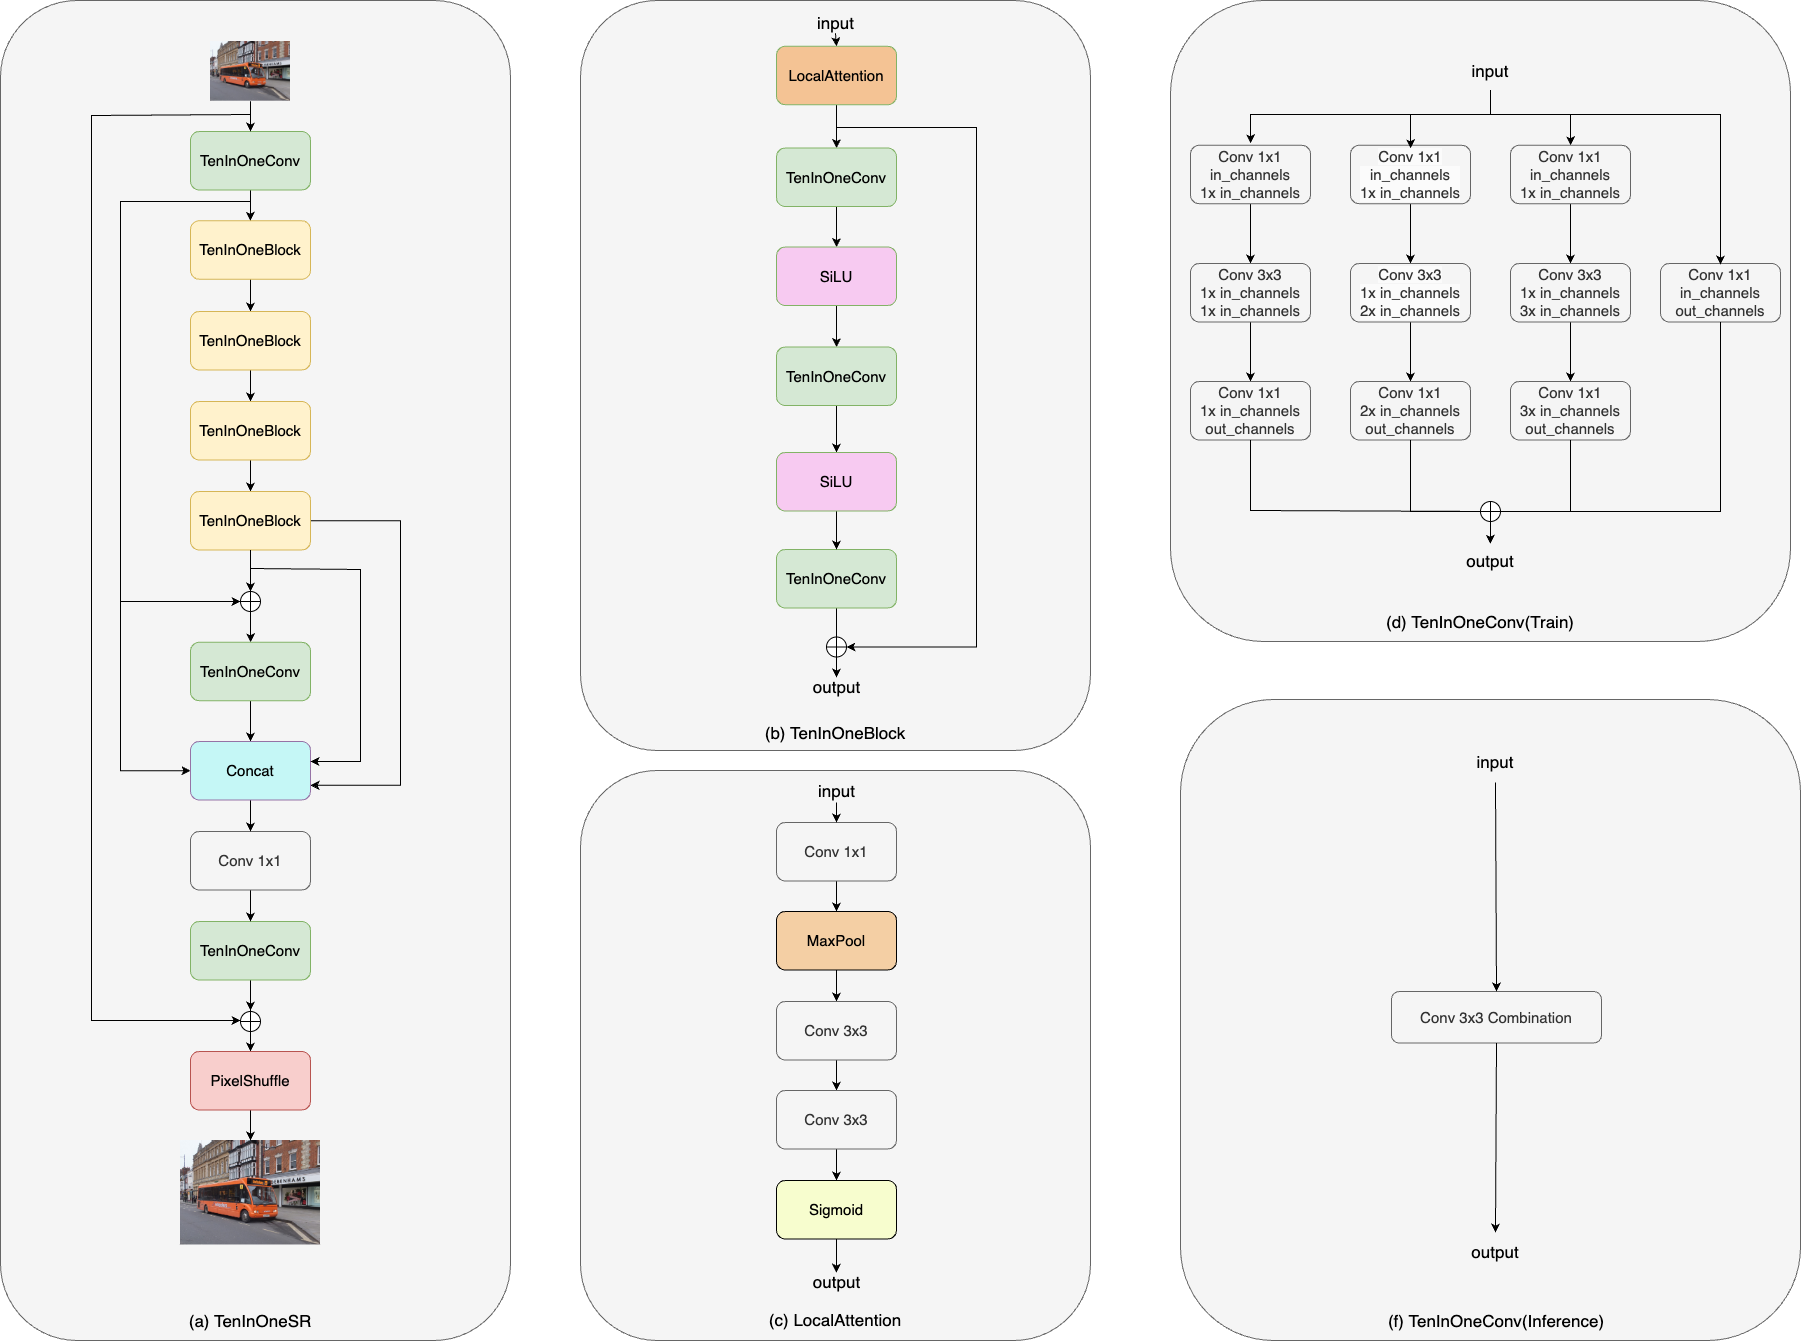
\includegraphics[width=\linewidth]{figure.png}
  \caption{The architecture of our proposed TenInOneSR.}
  \label{fig:architecture}
\end{figure}


TenInOneSR employs four TenInOneBlock modules. Each of these blocks (detailed in Figure (b)) begins with a LocalAttention module, which enhancing the network’s ability to capture fine details. Subsequently, each block applies three cascaded TenInOneConv layers, interleaved with the SiLU activation function, to perform hierarchical feature refinement. The block concludes with a residual connection, allowing better gradient flow.

Notably, the behavior of the TenInOneConv differs between the training and inference phases. During training (Figure (d)), TenInOneConv operates in a multi-branch configuration. It introduces three parallel convolutional branches with different channel expansion ratios (gains set as 1, 2, and 3), along with an additional skip connection. This multi-scale feature extraction enables the network to better aggregate complementary spatial features.

In the inference stage (Figure (f)), for computational efficiency and faster runtime, these multiple convolution kernels are fused into a single equivalent convolution kernel. Specifically, the parallel branches and skip connection weights are mathematically combined to form one unified 3×3 convolutional kernel, significantly accelerating inference without compromising performance.

\textbf{Training Details. }  The proposed architecture is trained on two NVIDIA RTX Titan GPUs with a total of 48 GB memory. 

In the first training stage, the DIV2K dataset is augmented by a factor of 85$\times$ and registered into the LSDIR format, resulting in a large-scale training set containing 152{,}991 high-resolution RGB images. During this stage, training is conducted with 64 randomly cropped 256$\times$256 patches per batch, using common augmentations such as random flipping and rotation. The model is optimized using the Adam optimizer with L1 loss for a total of 100{,}000 iterations. The learning rate is initialized at 5$\times$10$^{-4}$ and decayed by half every 20{,}000 iterations.

In the second stage, we keep the training strategy and hyperparameters unchanged, except for increasing the input patch size to 384$\times$384 and reducing the batch size to 32 to fit GPU memory. Then another 100{,}000 training iterations are conducted to further improve the model’s performance on higher-resolution textures.

In the second stage, we keep the training strategy and hyperparameters unchanged, except for increasing the input patch size to 384×384 and reducing the batch size to 32 to fit GPU memory.Then another 100,000 training iterations are conducted to further improve the model’s performance on higher-resolution textures.


\section{Other details}
\begin{itemize}
\item Planned submission of a solution(s) description paper at NTIRE 2025 workshop.
\item General comments and impressions of the NTIRE 2025 challenge. 
\item What do you expect from a new challenge in image restoration, enhancement, and manipulation?
\item Other comments: encountered difficulties, fairness of the challenge, proposed subcategories, proposed evaluation method(s), etc.
\end{itemize}

%%%%%%%%% REFERENCES
{\small
\bibliographystyle{ieee_fullname}
\bibliography{egbib}
}

\end{document}